\documentclass[11pt,preprint, authoryear]{elsarticle}

\usepackage{lmodern}
%%%% My spacing
\usepackage{setspace}
\setstretch{1}
\DeclareMathSizes{12}{14}{10}{10}

% Wrap around which gives all figures included the [H] command, or places it "here". This can be tedious to code in Rmarkdown.
\usepackage{float}
\let\origfigure\figure
\let\endorigfigure\endfigure
\renewenvironment{figure}[1][2] {
    \expandafter\origfigure\expandafter[H]
} {
    \endorigfigure
}

\let\origtable\table
\let\endorigtable\endtable
\renewenvironment{table}[1][2] {
    \expandafter\origtable\expandafter[H]
} {
    \endorigtable
}


\usepackage{ifxetex,ifluatex}
\usepackage{fixltx2e} % provides \textsubscript
\ifnum 0\ifxetex 1\fi\ifluatex 1\fi=0 % if pdftex
  \usepackage[T1]{fontenc}
  \usepackage[utf8]{inputenc}
\else % if luatex or xelatex
  \ifxetex
    \usepackage{mathspec}
    \usepackage{xltxtra,xunicode}
  \else
    \usepackage{fontspec}
  \fi
  \defaultfontfeatures{Mapping=tex-text,Scale=MatchLowercase}
  \newcommand{\euro}{€}
\fi

\usepackage{amssymb, amsmath, amsthm, amsfonts}

\def\bibsection{\section*{References}} %%% Make "References" appear before bibliography


\usepackage[round]{natbib}

\usepackage{longtable}
\usepackage[margin=2.3cm,bottom=2cm,top=2.5cm, includefoot]{geometry}
\usepackage{fancyhdr}
\usepackage[bottom, hang, flushmargin]{footmisc}
\usepackage{graphicx}
\numberwithin{equation}{section}
\numberwithin{figure}{section}
\numberwithin{table}{section}
\setlength{\parindent}{0cm}
\setlength{\parskip}{1.3ex plus 0.5ex minus 0.3ex}
\usepackage{textcomp}
\renewcommand{\headrulewidth}{0.2pt}
\renewcommand{\footrulewidth}{0.3pt}

\usepackage{array}
\newcolumntype{x}[1]{>{\centering\arraybackslash\hspace{0pt}}p{#1}}

%%%%  Remove the "preprint submitted to" part. Don't worry about this either, it just looks better without it:
\makeatletter
\def\ps@pprintTitle{%
  \let\@oddhead\@empty
  \let\@evenhead\@empty
  \let\@oddfoot\@empty
  \let\@evenfoot\@oddfoot
}
\makeatother

 \def\tightlist{} % This allows for subbullets!

\usepackage{hyperref}
\hypersetup{breaklinks=true,
            bookmarks=true,
            colorlinks=true,
            citecolor=blue,
            urlcolor=blue,
            linkcolor=blue,
            pdfborder={0 0 0}}


% The following packages allow huxtable to work:
\usepackage{siunitx}
\usepackage{multirow}
\usepackage{hhline}
\usepackage{calc}
\usepackage{tabularx}
\usepackage{booktabs}
\usepackage{caption}


\newenvironment{columns}[1][]{}{}

\newenvironment{column}[1]{\begin{minipage}{#1}\ignorespaces}{%
\end{minipage}
\ifhmode\unskip\fi
\aftergroup\useignorespacesandallpars}

\def\useignorespacesandallpars#1\ignorespaces\fi{%
#1\fi\ignorespacesandallpars}

\makeatletter
\def\ignorespacesandallpars{%
  \@ifnextchar\par
    {\expandafter\ignorespacesandallpars\@gobble}%
    {}%
}
\makeatother

\newenvironment{CSLReferences}[2]{%
}

\urlstyle{same}  % don't use monospace font for urls
\setlength{\parindent}{0pt}
\setlength{\parskip}{6pt plus 2pt minus 1pt}
\setlength{\emergencystretch}{3em}  % prevent overfull lines
\setcounter{secnumdepth}{5}

%%% Use protect on footnotes to avoid problems with footnotes in titles
\let\rmarkdownfootnote\footnote%
\def\footnote{\protect\rmarkdownfootnote}
\IfFileExists{upquote.sty}{\usepackage{upquote}}{}

%%% Include extra packages specified by user
\usepackage{booktabs}
\usepackage{longtable}
\usepackage{array}
\usepackage{multirow}
\usepackage{wrapfig}
\usepackage{float}
\usepackage{colortbl}
\usepackage{pdflscape}
\usepackage{tabu}
\usepackage{threeparttable}
\usepackage{threeparttablex}
\usepackage[normalem]{ulem}
\usepackage{makecell}
\usepackage{xcolor}

%%% Hard setting column skips for reports - this ensures greater consistency and control over the length settings in the document.
%% page layout
%% paragraphs
\setlength{\baselineskip}{12pt plus 0pt minus 0pt}
\setlength{\parskip}{12pt plus 0pt minus 0pt}
\setlength{\parindent}{0pt plus 0pt minus 0pt}
%% floats
\setlength{\floatsep}{12pt plus 0 pt minus 0pt}
\setlength{\textfloatsep}{20pt plus 0pt minus 0pt}
\setlength{\intextsep}{14pt plus 0pt minus 0pt}
\setlength{\dbltextfloatsep}{20pt plus 0pt minus 0pt}
\setlength{\dblfloatsep}{14pt plus 0pt minus 0pt}
%% maths
\setlength{\abovedisplayskip}{12pt plus 0pt minus 0pt}
\setlength{\belowdisplayskip}{12pt plus 0pt minus 0pt}
%% lists
\setlength{\topsep}{10pt plus 0pt minus 0pt}
\setlength{\partopsep}{3pt plus 0pt minus 0pt}
\setlength{\itemsep}{5pt plus 0pt minus 0pt}
\setlength{\labelsep}{8mm plus 0mm minus 0mm}
\setlength{\parsep}{\the\parskip}
\setlength{\listparindent}{\the\parindent}
%% verbatim
\setlength{\fboxsep}{5pt plus 0pt minus 0pt}



\begin{document}



\begin{frontmatter}  %

\title{Much Ado About Dividends}

% Set to FALSE if wanting to remove title (for submission)




\author[Add1]{Gabriel Rambanapasi}
\ead{gabriel.rams44@gmail.com}





\address[Add1]{Stellenbosch University, Cape Town, South Africa}

\cortext[cor]{Corresponding author: Gabriel Rambanapasi}

\begin{abstract}
\small{
This paper investigates dividends return predictive signals, focusing on
Dividend Yield (DY) and Dividend Growth (DG) signals, within both
domestic and international contexts. Over an extended investment
horizon, dividend portfolios consistently exhibit positive excess
returns, with notable variations across regional indexes. Notably, these
portfolios demonstrate capital protection during periods of heightened
market volatility, particularly the DY strategies. Surprisingly, South
African portfolios perform well during market turbulence, a departure
from the typical flight to safety. In contrast, during interest rate
cycles, all strategies perform optimally in low-interest-rate
environments. Information ratio analysis highlights that dividend
strategies do not uniformly maintain positive ratios, with varying
performance patterns across different regions. When integrated with
drawdown analysis, advanced economies exhibit lower systematic risk,
while South African and Emerging Market drawdowns suggest reduced
systematic risk in these markets. Within the South African context,
dividend portfolios display potential value during high volatility and
rising interest rate cycles, though P/E-based portfolios outperform them
in other scenarios. Consequently, dividend portfolios may not be an
ideal proxy for value. Investors with specific preferences may still
find value in these strategies, but for those constrained by investment
policy statements, DG portfolios offer practical, lower-volatility
alternatives to achieve returns akin to the market index. This study
contributes insights into dividend portfolio dynamics, enabling
investors to make informed choices based on their objectives and
constraints.
}
\end{abstract}

\vspace{1cm}





\vspace{0.5cm}

\end{frontmatter}

\setcounter{footnote}{0}



%________________________
% Header and Footers
%%%%%%%%%%%%%%%%%%%%%%%%%%%%%%%%%
\pagestyle{fancy}
\chead{}
\rhead{}
\lfoot{}
\rfoot{\footnotesize Page \thepage}
\lhead{}
%\rfoot{\footnotesize Page \thepage } % "e.g. Page 2"
\cfoot{}

%\setlength\headheight{30pt}
%%%%%%%%%%%%%%%%%%%%%%%%%%%%%%%%%
%________________________

\headsep 35pt % So that header does not go over title




\hypertarget{introduction}{%
\section*{Introduction}\label{introduction}}
\addcontentsline{toc}{section}{Introduction}

This paper aims to investigate the return predictive signal of
dividend-paying stocks. The value of dividends to shareholders has long
been a subject of debate among academics and practitioners, with
evidence both for their relevance and irrelevance. Miller \& Modigliani
(\protect\hyperlink{ref-miller}{1961}) proposed the dividend irrelevance
theorem, which argues that dividend payments are irrelevant because they
do not affect shareholder wealth, as it is the income a firm generates
that impacts wealth, not the way the firm distributes that income. In
contrast, Gordon (\protect\hyperlink{ref-gordon1962}{1962}) argued that
investors should prefer cash flows because they are certain, as opposed
to the riskier capital gains. According to this theory, the ``Bird in
Hand Theorem'' is used to justify the demand for dividend stocks,
especially for less risk-tolerant investors. Moreover, a closer
examination of the Miller \& Modigliani
(\protect\hyperlink{ref-miller}{1961}) theory reveals unrealistic
assumptions, rendering arguments immaterial once real-world constraints,
such as taxes, transaction costs, and behavioral biases, are considered.
Consequently, theories that consider information asymmetries, tax
considerations, and signaling provide convincing arguments for the
relevance of dividend payments in addressing real-world considerations.
Campbell (2017) posits that the value of a stock is a function of its
future cash flow. If markets are assumed to be efficient, then companies
that do not pay dividends should have a value of zero unless there is an
expectation of future receipts from the investment in said company.
Therefore, we can safely assume a direct relationship between share
price and new information that affects future cash flows. Event studies
on various types of dividend payments address this, and it is often
noted that the payment of dividends leads to a decrease in stock prices
and thus stock valuation. Suwanna (2012) demonstrates that dividend
announcements decrease share prices by the value of the dividend. This
could be because dividends are a capital budgeting decision, and their
payment reduces retained earnings, consequently affecting the share
price.

This study provides an extensive investigation into the return signaling
of dividend portfolios. Firstly, it reviews existing literature on
dividend payments, their rationale, and the theories both for and
against their relevance. Secondly, it outlines our methodology for
constructing dividend portfolios, which includes our utility optimizer
and associated constraints. Thirdly, the study discusses the results by
addressing the first question: When do dividend signals work? To answer
this, we initially examine the cumulative excess returns offered by
global dividend indexes to provide a comprehensive overview of the
performance of geographical dividend portfolios. Our analysis shows that
dividend portfolios, whether high yield (HY) or dividend growth (DG), do
not consistently provide a clear signal for returns. However, when we
stratify our sample according to interest rate cycles (Hiking, Cutting,
and Neutral) and market regimes (High and Low Volatility), unique to
each geographical region, we begin to find that within specific market
regimes, dividend signals exhibit defensive characteristics and offer
higher excess returns during periods of High Volatility. This, however,
does not guarantee positive returns for all indexes, as our proxies for
the United States (US) HY, UK HY, and World indexes returned negative
results over their respective periods.

Regarding performance consistency, when examining the rolling
information ratio, we observe an inherent lack of consistency in
dividend portfolio performance, with most strategies underperforming the
benchmark over the past 15 years. Nevertheless, coupled with drawdowns
experienced in different jurisdictions, we acknowledge that advanced
market dividend portfolios experience the least variation in drawdowns
compared to emerging markets. The results indicate that both growth and
high-yield dividend portfolios tend to underperform relative to their
benchmarks, raising questions about their ability to extract a value
premium.

Lastly, the paper delves into how dividend portfolios work with the goal
of constructing a portfolio that can best harness the existing premium.
We utilize share data from the Johannesburg Stock Exchange (JSE), with
our benchmark being the Capped SWIX Top 50. We construct four portfolios
using 3-month and 9-month measures of HY, 1 and 3-year DG measures,
together with price momentum and dividend coverage ratios. Similar to
the analysis of international dividend portfolios, our portfolios
exhibit defensive properties in high-volatility periods but fail to
consistently capture a premium over investing in a market index.
\newpage

\hypertarget{literature-review}{%
\section{Literature Review}\label{literature-review}}

\hypertarget{introduction-1}{%
\subsection{Introduction}\label{introduction-1}}

This literature review delves into the popular theories behind the
rationale of dividends issuance. We first unpack dividend theorems
whilst juxtaposing with empirical evidence to reveal the information
content within the issuance of dividends. Our review of emprical
literature unveils a paradox, where market prices exhibit less decline
than the theoretical prescription once we consider real world
constraints investing. This phenomenon hints at concealed market
frictions, suggesting that dividends might indeed carry valuable
information content.Subsequently we discuss studies that opine these
market frictions to come from stock liquidity, differences in taxes on
dividends and captial gains, and signaling effects. The literature is
inconclusive however we conjuncture that to discern the true
informational value, a thorough examination of individual dividend
policy relative to company fundamentals is crucial. To get a general
signal we explore various literature employ systematic approach to
determine wheter dividends provide a return invest cue.

\hypertarget{dividend-theories}{%
\subsection{\texorpdfstring{Dividend Theories
\label{theory}}{Dividend Theories }}\label{dividend-theories}}

The debate surrounding the irrelevance of dividends pioneered by Miller
\& Modigliani (\protect\hyperlink{ref-miller}{1961}), gave insight into
firm valuation. He posited that in a perfect market, one that is devoid
od market frictions and transaction costs, investors should be
indifferent to receiving dividends, as firm value is derived from
earning which result from investment policy. They reinforced the
dividend irrelevance theorem by arguing that if the dividend practice
adopted by any firm corresponds to the dividend preference of its
shareholders each firm would attract its clientele based on its dividend
policy practice. Moreover given their assumptions, a change in dividend
policy will not materially affect any firm valuation because with the
existence of several competing firms, a firm that changes dividend
policy may not act by the preference of some shareholder simply induce a
movement across firms as investors try to align with firms whose
dividend practice corresponds with their dividend preference.
Consequently, in the long run, equilibrium in terms of choice of
investment and dividend preference will be attained and shareholders
valuation of the firm will not be different from those of firms with
different dividend policy.

Miller \& Modigliani (\protect\hyperlink{ref-miller}{1961}) shortfalls
in unrealistic real world assumptions resulted in opposing arguments.
The bird in the hand theory a common argument that is used to make a
case for investor preferences for dividend payment, Walter
(\protect\hyperlink{ref-walter1963dividend}{1963}) suggests that
investors prefer dividends to capital gains because the nature payment
of dividends effectively guarantees income towards investors against
some probability of receiving capital gains at some point during an
investment holding period. This implies that investors prefer to receive
dividends now so that they can reinvest and earn a further return.
Buttressing this, Lintner
(\protect\hyperlink{ref-lintner1956distribution}{1956}) argued that
dividend are desired because it helps to reduce the level of information
asymmetry, a firm that pays dividend assures investors that the firm is
performing well. Moreover, Gordon
(\protect\hyperlink{ref-gordon1963optimal}{1963}) saw dividend as
preferred to capital gains because dividend payment reduces risks
associated with investments because it is more certain. Therefore, the
major implication of the bird in the hand theory sees risk in the
reinvestment of company profits through keeping it as retained earning.
Consequently, investors expect a higher expected return with the payment
of dividend which ultimately raises the costs of capital from investors.

Lintner (\protect\hyperlink{ref-lintner1956distribution}{1956})
suggested that information asymmetry between shareholders and
management, brings into focus management decisions and their impact on
firm prospects. Cognizant of this, managers of dividend paying companies
are more willing to raise rather than reduce dividend levels, and this
is construed to mean that given dividend payment history decreases are
associated with negative signals while dividend increases signal
positive news signal positive news. Bhattacharyya
(\protect\hyperlink{ref-bhattacharyya2007dividend}{1979}), presents a
signaling model where the liquidation of the firm is related to the
actual dividend paid and any change in dividend alters the liquidation
value of the firm. The liquidation value represents the amount of money
shareholders would receive if the company were to be dissolved, of which
dividends can affect this value by depleting the firm's cash reserves by
distributing earnings to shareholders. The distribution the firm reduces
its financial cushion during financial hardships. Consequently, dividend
payments can influence investors' perceptions of the firm's risk profile
and future prospects.Changes in dividend under the signalling model
convey important information about a firm's outlook. for the quality of
firms assets.

Jensen \& Meckling (\protect\hyperlink{ref-jensen1976theory}{1976})
argued for agency costs, managerial behavior and ownership structure in
advocating for the relevance of dividend payments. The separation of
control and ownership gives rise to a principle-agent problem because
managers have the responsibility of acting in the best interest of the
owners, however, there are possibilities for conflicts between the
managers and shareholders. A high level of retained may motivate
managers to pursue decisions that promote their own self interests,
therefore shareholders mimimize the amount of retained earnings on hand
available to managers to mitigate the risk of acting out of self
interest. Jensen \& Meckling
(\protect\hyperlink{ref-jensen1976theory}{1976}) proposes a free cash
flow model that states ``when a firm has financed all its positive net
present value investments, it should distribute all its free cash flow
as dividends''. This prescription should reduce agency costs.

\hypertarget{empirical-studies-and-their-return-predictive-signal}{%
\subsection{Empirical studies and their return predictive
signal}\label{empirical-studies-and-their-return-predictive-signal}}

Empirical studies we aseesss are concerned with finding factors that
influence dividend policy, thus relating them underlying theories in
section \ref{theory}. Baker \& Wurgler
(\protect\hyperlink{ref-baker2006investor}{2006}) show that investor
sentiment is a significant determinant of dividend policy. Their study
suggests that waves of investor sentiment have differential effects on
stock returns, particularly for stock that are difficult to arbitrage
and have valuations that are highly subjective. In reaction, management
may adjust their dividend policy in response to prevailing market
sentiment, potentially paying dividends to signal confidence during
periods of high sentiment and conserving cash during times of market
uncertainty. With regard to category of stock and performance, they also
find that during periods of low sentiment, returns are high for small
size, young firms, unprofitable stock, non dividend paying, extreme
growth and distressed stocks. During periods of high sentiment this
group of stock experiences low returns.

Grullon, Larkin \& Michaely
(\protect\hyperlink{ref-grullon2019dividend}{2019}) analyse managerial
decisions to distribute cash flows in industries with varying levels of
competitiveness.Albeit this study was conducted in the manufacturing
sector,its insights indicates that firms operating in competitive
industries tend to have lower payout ratios.Thus firms in highly
competitive environments prioritize investment and innovation over
dividend payments, moreover whose overall characteristics suggest that
lower agency costs and less likely to be a target of predation.
Interestingly, the authors allude to disciplinary forces that follow
Jensen \& Meckling (\protect\hyperlink{ref-jensen1976theory}{1976}) free
cash flow theory, that is, managers in competitive industries payout
excess cash and with the idea that corporate payouts are the ``outcome''
of external factors. Denis \& Osobov
(\protect\hyperlink{ref-denis2008firms}{2008}) provide cross-country
evidence on the determinants of dividend policy, revealing that larger,
more profitable firms with higher retained earnings are more likely to
pay dividends across US, Canada, UK, Germany, France, and Japan. In each
country, aggregate dividend payments concentrated among the largest,
most profitable firms. Outside of the US there is little evidence of a
systematic positive relation between relative prices of dividend paying
and non-paying firms and the propensity to pay dividends. These
reconcile with Jensen \& Meckling
(\protect\hyperlink{ref-jensen1976theory}{1976}) \& Lintner
(\protect\hyperlink{ref-lintner1956distribution}{1956}) as these studies
posit that firms with strong financial performance and stability are
more inclined to pay dividends to signal quality and mitigate agency
conflicts.

Baker \& Wurgler (\protect\hyperlink{ref-baker2006investor}{2006}),
Grullon \emph{et al.}
(\protect\hyperlink{ref-grullon2019dividend}{2019}) \& Denis \& Osobov
(\protect\hyperlink{ref-denis2008firms}{2008}) show that dividend paying
companies usually comprise of larger more profitable firms. An intuitive
proxy for why companies with high dividend yields might outperform their
more miserly counterparts, is that dividend yield proxies for the Value
factor (\protect\hyperlink{ref-basu1977investment}{Basu, 1977}).
Consider the equation below:

\begin{align*}
DY = \frac{EPS}{\text{Price}} \times \text{Payout Ratio}
\end{align*}

Assuming a constant payout ratio, dividend yield (DY) would simply
become a function of changes in earnings yield. From the equation,
holding earnings per share (EPS) constant, price has a inverse relation
to DY. This implies that studies identifying return predictive signal DY
verify the existence of the value-signal \footnote{Value as an
  investment factor dates back to Basu (1977), who used the
  price-earnings ratio of companies to compare stock performance. Since
  then, many studies have confirmed the existence of a value premium,
  where cheap stocks outperform their more expensive counterparts over
  time.}. Notably, Cornell
(\protect\hyperlink{ref-cornell2014dividend}{2014}) studied the
predictive power of dividend-price ratios using US data. The findings
revealed that higher dividend-price ratios are associated with higher
future stock returns, suggesting stock-return predictability based on
dividend-price ratios. This implies that investors may be able to
leverage dividend-price ratios as an informational tool to make informed
investment decisions and potentially earn above-average returns.
Similarly, Conover, Jensen \& Simpson
(\protect\hyperlink{ref-conover2016difference}{2016}) explored the
investment benefits of dividend-paying stocks by analyzing dividend
yield and its correlation with stock returns. The study uncovered that
high-dividend-paying stocks tend to exhibit lower risk and higher
returns compared to non-dividend-paying stocks. Specifically,
high-dividend payers outperformed non-dividend payers by over 1.5\% per
year on average. Other studies used growth in dividends to capture
second order characteristics of dividend payers, Chen
(\protect\hyperlink{ref-chen2009reversal}{2009}) delved into the
predictive power of dividend growth for future stock returns, focusing
on historical data from the prewar period of the early 1900s. The study
identified strong predictive power in dividend growth during this
historical period, suggesting that changes in dividend growth rates can
serve as valuable signals for predicting future stock returns. However,
the predictive power of dividend growth appeared to diminish in the
postwar years, highlighting the importance of historical context and
market dynamics in assessing the effectiveness of dividend-based
investment strategies.

\newpage

\hypertarget{data-and-methodology}{%
\section*{Data and Methodology}\label{data-and-methodology}}
\addcontentsline{toc}{section}{Data and Methodology}

\hypertarget{data-for-globally-traded-dividend-indexes}{%
\subsection{\texorpdfstring{Data for Globally Traded Dividend
Indexes\label{int}}{Data for Globally Traded Dividend Indexes}}\label{data-for-globally-traded-dividend-indexes}}

We use historical price data for globally traded dividend indexes in
Table \ref{tabdes} from January 1 2003 to January 1 2023, a 20 year
sample period. All of the studied indexes are constructed in gross total
return in the same currency. Full descriptions on benchmark, dividend
indexes are given in Table \ref{tabdes}. Our metric of interest are
annualized excess returns of individual indexes to their respective
benchmarks following Bacon
(\protect\hyperlink{ref-bacon2023practical}{2023}). To achieve this we
scale observations to an annual scale by raising the compound return to
the number of periods in a year, following this we take the root of
total observations: \begin{align*}
\operatorname{Annualized Return} & = \sqrt[n]{\operatorname{prod}\left(1+R_a\right)^{\operatorname{scale}}} - 1
\end{align*} where \(R_a\) is the return on the asset, \(scale\) is the
number of periods in a year, \(n\) is the total number of periods.
Following this, we simply take the difference of annualized return to
get our excess return: \begin{align*}
E R_a = R_{a} - R_{b}
\end{align*} where \(R_{a}\) are annualized return on the asset and
\(R_{b}\) are annualized return of the benchmark. From our excess return
metrics, we calculate second moments and third moments to describe
distributional properties. Moreover we make other transformations to our
international portfolio sample to get a nuanced perspective on
performance during different time periods. For interest rate regime
cycles we use interest rate schedules from central banks of country of
domicile for the index. That is, to proxy periods of high and low
interest rates we stratify our sample interest rate hiking and cutting
cycles where periods of sustained changes rate changes occur at least
every five quarters. Likewise, we use proxies for volatility such as the
VIX index in the United States, V2X in Europe and JALSH RV in South
Africa that consider implied and realized equity market volatilities to
proxy for different periods of market stability. After stratification,
we geometrically chain the excess returns for the different periods
before annualizing. To stratify amount of daily data for the respective
interest rate cycles has to be large enough to annualized, however, if
our proxies for volatility breach the top or bottom quintile for less
than 50 trading days, the period is excluded in order to avoid
annualizing small frequencies.

\hypertarget{local-dividend-portfolios}{%
\subsection{Local Dividend Portfolios}\label{local-dividend-portfolios}}

We use historical daily price data in table \ref{tabdes} from January 1
2003 to July 7 2023, a roughly 20 year sample period for equity listed
in the Johannesburg Stock Exchange and retrieve dividend yield ratios,
dividend cover ratio, price momentum, price to earnings ratio, dividend
growth per share from Bloomberg. We construct our portfolios using
signals on fundamental ratios and price momentum that are a blend of our
selected ratios as described in Table \ref{signal} below.

Our dividend portfolios are constructed by feeding into the optimizer
ranked signals, of which the optimizer does a aplha transformation on
the signal. Our optimizer makes slight modifications to the mean
variance portfolio that considers risk preferences of investors
(\protect\hyperlink{ref-markowitz1959portfolio}{Markowitz, 1959}). Risk
of \(n\) assets is defined \(\sigma^2\) based on individual asset
returns \(R_a\). We decompose returns into common factor \(X_f\) and
specific return \(u\). Our covariance matrix is then defined as: \[
\begin{aligned}
XFX^T + D
\end{aligned}
\] where: \begin{align*}
X & : n \times k \text{ matrix of asset exposures to the factors,} \\ F & : k \times k \text{ positive semi-definite factor covariance matrix, and} \\ D & : n \times n \text{ positive semi-definite covariance matrix representing a forecast of asset-specific risk.}
\end{align*} For optimization purposes, our \(\sigma^2\)) is considered
in two forms: total risk, where only portfolio holdings are considered
(benchmark holdings are irrelevant for the optimization process), and
active risk, which takes into account the difference between portfolio
holdings and benchmark holdings defined as: \begin{align*}
\text{Total Risk:} & \quad h^T(\lambda_F X F X^T + \lambda_D D) h \\
\text{Active Risk:} & \quad (h - h_B)^T(\lambda_F X F X^T + \lambda_D D)(h - h_B)
\end{align*} where: \begin{align*}
\lambda_F & : \text{common factor risk aversion parameter,} \\
\lambda_D & : \text{ specific risk aversion parameter,} \\
h & : n \times 1 \text{ vector of managed portfolio's holdings, and} \\
h_B & : n \times 1 \text{ vector of normal (benchmark) portfolio's holdings}
\end{align*}

The following accounts for practical considerations in constructing our
portfolios. We use the Capped SWIX as our benchmark and \(\lambda_F\)
and \(\lambda_D\) are set to 0.0075 and 1, respectively, with active
risk have an upper limit of 5\%. For our box constraints, sector
exposure can deviate from a range of 10\% relative to the Capped SWIX
and individual asset exposure is limited to 15\%. Our portfolio turnover
is limited to 10\% and we exclude the property sector from our
portfolios. \newpage

\hypertarget{results}{%
\section*{Results}\label{results}}
\addcontentsline{toc}{section}{Results}

\begin{itemize}
\tightlist
\item
  risk and return analsysis of internationally traded portfolios, this
  is to find out how they have performed over their market indxes.
\end{itemize}

\begin{longtable}{rrlrr}
\caption{First and Second Moments of Globally traded Dividend Portfolios \label{tab1}} \\ 
  \hline
 & date & Index & excess\_return & te \\ 
  \hline
1 & 1672358400.00 & FUDP & -8.41 & 7.95 \\ 
  2 & 1672358400.00 & M2GBDY & -1.49 & 8.57 \\ 
  3 & 1672358400.00 & M2WDHDVD...12 & -0.39 & 6.39 \\ 
  4 & 1672358400.00 & SPDAEET & 0.78 & 6.84 \\ 
  5 & 1672358400.00 & SPDAUDT & 1.64 & 5.59 \\ 
  6 & 1672358400.00 & SPJXDAJT & -1.19 & 15.07 \\ 
  7 & 1672358400.00 & SPSADAZT & -3.80 & 19.54 \\ 
  8 & 1672358400.00 & TJDIVD & -2.39 & 19.81 \\ 
   \hline
\hline
\end{longtable}

\begin{itemize}
\tightlist
\item
  cumulative returns
\end{itemize}

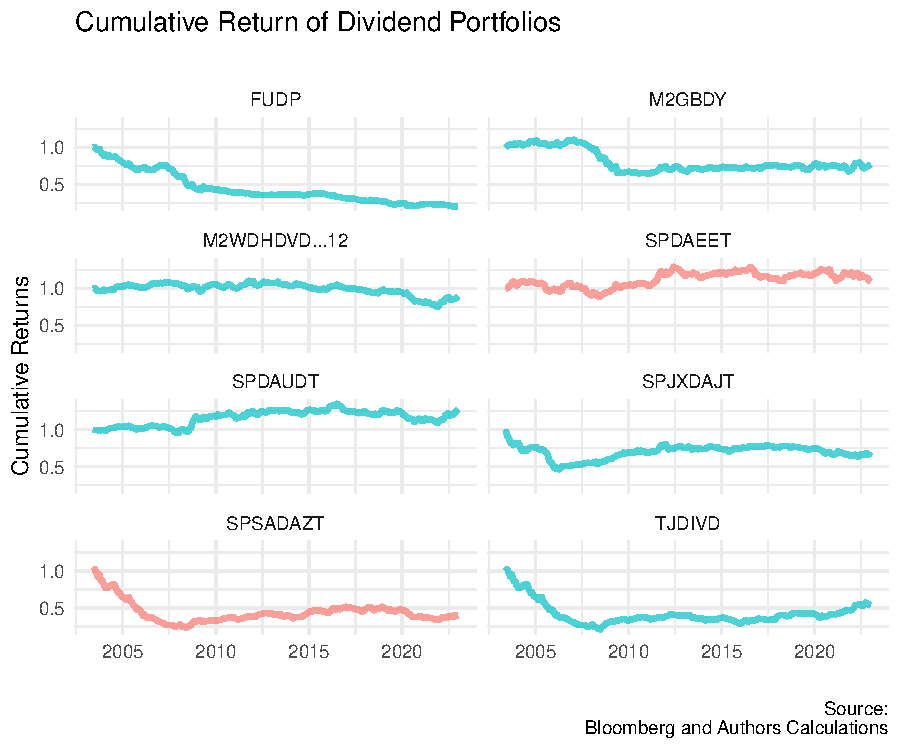
\includegraphics{MuchAdoDivs_files/figure-latex/unnamed-chunk-2-1.pdf}

\begin{itemize}
\tightlist
\item
  stratification results
\end{itemize}

\begin{tabular}{rllrrll}
  \hline
 & index & Cycle & Months & Ann Ret & Country & Signal \\ 
  \hline
1 & FUDP & High Vol &  20 & -2.84 & US & DY \\ 
  2 & M2GBDY & High Vol &  14 & -12.62 & UK & HY \\ 
  3 & M2WDHDVD...12 & High Vol &  14 & -8.47 & UK & HY \\ 
  4 & SPDAEET & High Vol &   7 & 24.52 & EU & DGPS \\ 
  5 & SPDAUDT & High Vol &  14 & -3.45 & UK & UK \\ 
  6 & SPJXDAJT & High Vol &  20 & -0.70 & JP & HY \\ 
  7 & SPSADAZT & High Vol &  17 & 14.43 & SA & DGPS \\ 
  8 & TJDIVD & High Vol &  17 & 18.90 & SA & HY \\ 
   \hline
\end{tabular}
\begin{longtable}{rllrrll}
\caption{Low Market Volatility Perfromance \label{tab2}} \\ 
  \hline
 & index & Cycle & Months & Ann Ret & Country & Signal \\ 
  \hline
1 & FUDP & lo Vol &   9 & -14.22 & US & DY \\ 
  2 & M2GBDY & lo Vol &   7 & -2.11 & UK & HY \\ 
  3 & M2WDHDVD...12 & lo Vol &   7 & -4.04 & UK & HY \\ 
  4 & SPDAEET & lo Vol &   4 & -15.73 & EU & DGPS \\ 
  5 & SPDAUDT & lo Vol &   7 & 0.08 & UK & UK \\ 
  6 & SPJXDAJT & lo Vol &   9 & -28.43 & JP & HY \\ 
  7 & SPSADAZT & lo Vol &   9 & 5.84 & SA & DGPS \\ 
  8 & TJDIVD & lo Vol &   9 & 27.37 & SA & HY \\ 
   \hline
\hline
\end{longtable}
\begin{longtable}{rllrrll}
\caption{Cutting Cycle Annualized Returns  \label{tab1}} \\ 
  \hline
 & index & Cycle & Months & Ann Ret & Country & Signal \\ 
  \hline
1 & FUDP & lo Vol &   9 & -14.22 & US & DY \\ 
  2 & M2GBDY & lo Vol &   7 & -2.11 & UK & HY \\ 
  3 & M2WDHDVD...12 & lo Vol &   7 & -4.04 & UK & HY \\ 
  4 & SPDAEET & lo Vol &   4 & -15.73 & EU & DGPS \\ 
  5 & SPDAUDT & lo Vol &   7 & 0.08 & UK & UK \\ 
  6 & SPJXDAJT & lo Vol &   9 & -28.43 & JP & HY \\ 
  7 & SPSADAZT & lo Vol &   9 & 5.84 & SA & DGPS \\ 
  8 & TJDIVD & lo Vol &   9 & 27.37 & SA & HY \\ 
   \hline
\hline
\end{longtable}
\begin{longtable}{rllrrll}
\caption{Hiking Cycle Annualized Returns  \label{tab1}} \\ 
  \hline
 & index & Cycle & Months & Ann Ret & Country & Signal \\ 
  \hline
1 & FUDP & Hiking &  29 & -15.70 & US & Dividend Yield \\ 
  2 & M2GBDY & Hiking &  29 & -1.74 & UK & Dividend Yield \\ 
  3 & M2WDHDVD...12 & Hiking &  29 & 3.83 & UK & Dividend Yield \\ 
  4 & SPDAEET & Hiking &  26 & 1.08 & EU & Dividend Growth Per Share \\ 
  5 & SPDAUDT & Hiking &  29 & 2.12 & UK & Dividend Yield \\ 
  6 & SPJXDAJT & Hiking &  35 & -8.43 & JP & Dividend Yield \\ 
  7 & SPSADAZT & Hiking &  38 & 1.54 & SA & Dividend Growth Per Share \\ 
  8 & TJDIVD & Hiking &  38 & -3.87 & SA & Dividend Yield \\ 
   \hline
\hline
\end{longtable}

\newpage

\hypertarget{conclusion}{%
\section*{Conclusion}\label{conclusion}}
\addcontentsline{toc}{section}{Conclusion}

Over the course of time, dividend portfolios, encompassing both DY and
DG strategies, have consistently displayed positive excess returns,
evident in the cumulative excess return figures. Although the UK\_HY
index notably exhibits the highest cumulative return, this trend is not
uniformly observed across various regional indexes. However, when we
segment these portfolios based on different periods of market
volatility, a distinct pattern emerges. During phases of heightened
market volatility, dividend strategies prove to be effective in
providing capital protection when integrated into a diversified asset
portfolio. Furthermore, during such high volatility periods, DY
strategies outperform the DG strategies. An intriguing observation is
that South African portfolios tend to perform well during these high
volatility periods, which is somewhat unconventional, given that such
times are typically associated with a flight to safety. Emerging Markets
(EM) and, by extension, South Africa, are generally perceived as riskier
investments.

Expanding our analysis to incorporate interest rate cycles reveals a
contrasting effect compared to the volatility-based stratification. It
becomes evident that all strategies tend to yield the highest returns
during low interest rate cycles. Information ratio analysis indicates
that dividend strategies generally do not exhibit consistent return
performance. At a broader level, these portfolios do not consistently
maintain a positive information ratio over an extended investment
horizon. However, disparities in performance emerge, with South African
dividend indexes consistently delivering positive ratios over the past
decade. Conversely, Emerging Markets and Japanese indexes have
experienced substantial declines in their information ratios, despite
seemingly consistent performance prior to 2015. Meanwhile, the United
States, European Union, and United Kingdom indexes have exhibited
unpredictable performance over the sampled period.

When we combine our information ratio findings with drawdown analysis,
we observe that advanced economies have experienced fewer drawdowns over
the sample period, with the exception of the UK. This could suggest a
relatively lower level of systematic risk in these economies.
Conversely, South African and Emerging Market drawdowns have been less
severe, possibly indicating reduced systematic risk in emerging markets.

In the context of South Africa, focusing on the top 50 companies by
market capitalization, we observe a performance pattern similar to our
international analysis. Firstly, dividend portfolios do not convincingly
deliver superior total returns, as calculated by cumulative returns.
However, their value becomes apparent during periods of high volatility
and rising interest rate cycles. Moreover, when we consider more
traditional proxies for value, such as the Price to Earnings (P/E)
ratio, the efficacy of dividend signals diminishes. In other words,
portfolios constructed based on P/E ratios perform exceptionally well in
our back-test and performance criteria, outperforming the market index
68.8\% of the time.

In conclusion, dividend portfolios may not serve as an ideal proxy for
value, and investors may benefit more from exploring investment products
that provide an income component to their total returns. However, it's
worth noting that investor preferences can vary, potentially driving
demand for specific dividend portfolio strategies. Based on the
evidence, investors constrained by investment policy statements may find
value in equity portfolios constructed using Dividend Growth (DG)
strategies as these use signals that do a better job of capturing
company cash flow management and managerial qualities. Despite their
lower hit rate, DG portfolios exhibit lower volatility in achieving
returns, making them a practical and profitable means of attaining
returns that closely align with the market index.

\newpage

\hypertarget{appendix}{%
\section*{Appendix}\label{appendix}}
\addcontentsline{toc}{section}{Appendix}

\begingroup\fontsize{8pt}{9pt}\selectfont
\begin{longtable}{llll}
  \toprule
TICKER & NAME & Codename & Inception Dates \\ 
  \hline 
\endhead 
\hline 
{\footnotesize Continued on next page} 
\endfoot 
\endlastfoot 
 \midrule
FUDP & FTSE UK Dividend+ Index & UK\_HY &  \\ 
  M2EFDY & MSCI EM HY Gross Total Return USD Index & EM\_HY &  \\ 
  M2GBDY & MSCI UK HY Gross Total Return USD Index & UK\_HY &  \\ 
  M2JPDY & MSCI Japan HY Gross Total Return USD & JP\_HY &  \\ 
  M2USADVD & MSCI USA HY Gross Total Return USD Index & US\_HY &  \\ 
  M2WDHDVD & MSCI World HY Gross Total Return Total Return USD Index & W\_HY &  \\ 
  SPDAEET & S\&P EU 350 Dividends Aristocrats Total Return Index & EU\_DG &  \\ 
  SPJXDAJT & S\&P/JPX Dividend Aristocrats Total Return Index & JP\_DG &  \\ 
  SPDAUDT & S\&P 500 Dividend Aristocrats Total Return Index & US\_DG &  \\ 
  SPSADAZT & S\&P South Africa Dividend Aristocrats Index ZAR Gross TR & SA\_DG &  \\ 
  TJDIVD & FTSE/JSE Dividend+ Index Total Return Index & SA\_HY &  \\ 
  M2EUGDY & MSCI Europe Ex UK HYGross Total Return USD Index & EU\_HY &  \\ 
  TUKXG & FTSE 100 Total Return Index GBP & UK &  \\ 
  GDUEEGF & MSCI Daily TR Gross EM USD & EM &  \\ 
  GDDUUK & MSCI UK Gross Total Return USD Index & UK\_B &  \\ 
  TPXDDVD & Topix Total Return Index JPY & JP &  \\ 
  GDDUUS & MSCI Daily TR Gross USA USD & US &  \\ 
  GDDUWI & MSCI Daily TR Gross World USD & W &  \\ 
  SPTR350E & S\&P Europe 350 Gross Total Return Index & EU\_2 &  \\ 
  SPXT & S\&P 500 Total Return Index & JP &  \\ 
  SPXT & S\&P 500 Total Return Index & US\_2 &  \\ 
  JALSH & FTSE/JSE Africa All Share Index & SA &  \\ 
  JALSH & FTSE/JSE Africa All Share Index & SA &  \\ 
  GDDUE15X & MSCI Daily TR Gross Europe Ex UK USD & EU &  \\ 
   \bottomrule
\caption{Index Description \label{tabdes}} 
\end{longtable}
\endgroup

\newpage

\hypertarget{references}{%
\section*{References}\label{references}}
\addcontentsline{toc}{section}{References}

\hypertarget{refs}{}
\begin{CSLReferences}{1}{0}
\leavevmode\vadjust pre{\hypertarget{ref-bacon2023practical}{}}%
Bacon, C.R. 2023. \emph{Practical portfolio performance measurement and
attribution}. John Wiley \& Sons.

\leavevmode\vadjust pre{\hypertarget{ref-baker2006investor}{}}%
Baker, M. \& Wurgler, J. 2006. Investor sentiment and the cross-section
of stock returns. \emph{The journal of Finance}. 61(4):1645--1680.

\leavevmode\vadjust pre{\hypertarget{ref-basu1977investment}{}}%
Basu, S. 1977. Investment performance of common stocks in relation to
their price-earnings ratios: A test of the efficient market hypothesis.
\emph{The journal of Finance}. 32(3):663--682.

\leavevmode\vadjust pre{\hypertarget{ref-bhattacharyya2007dividend}{}}%
Bhattacharyya, N. 1979. Dividend policy: A review. \emph{Managerial
Finance}. 33(1):4--13.

\leavevmode\vadjust pre{\hypertarget{ref-chen2009reversal}{}}%
Chen, L. 2009. On the reversal of return and dividend growth
predictability: A tale of two periods. \emph{Journal of Financial
Economics}. 92(1):128--151.

\leavevmode\vadjust pre{\hypertarget{ref-conover2016difference}{}}%
Conover, C.M., Jensen, G.R. \& Simpson, M.W. 2016. What difference do
dividends make? \emph{Financial Analysts Journal}. 72(6):28--40.

\leavevmode\vadjust pre{\hypertarget{ref-cornell2014dividend}{}}%
Cornell, B. 2014. Dividend-price ratios and stock returns: International
evidence. \emph{Journal of Portfolio management}. 40(2):122.

\leavevmode\vadjust pre{\hypertarget{ref-denis2008firms}{}}%
Denis, D.J. \& Osobov, I. 2008. Why do firms pay dividends?
International evidence on the determinants of dividend policy.
\emph{Journal of Financial economics}. 89(1):62--82.

\leavevmode\vadjust pre{\hypertarget{ref-gordon1962}{}}%
Gordon, M.J. 1962. The savings investment and valuation of a
corporation. \emph{The Review of Economics and Statistics}. 37--51.

\leavevmode\vadjust pre{\hypertarget{ref-gordon1963optimal}{}}%
Gordon, M.J. 1963. Optimal investment and financing policy. \emph{The
Journal of finance}. 18(2):264--272.

\leavevmode\vadjust pre{\hypertarget{ref-grullon2019dividend}{}}%
Grullon, G., Larkin, Y. \& Michaely, R. 2019. Dividend policy and
product market competition. \emph{Available at SSRN 972221}.

\leavevmode\vadjust pre{\hypertarget{ref-jensen1976theory}{}}%
Jensen, M.C. \& Meckling, W.H. 1976. Theory of the firm: Managerial
behavior, agency costs and ownership structure. \emph{Journal of
financial economics}. 3(4):305--360.

\leavevmode\vadjust pre{\hypertarget{ref-lintner1956distribution}{}}%
Lintner, J. 1956. Distribution of incomes of corporations among
dividends, retained earnings, and taxes. \emph{The American economic
review}. 46(2):97--113.

\leavevmode\vadjust pre{\hypertarget{ref-markowitz1959portfolio}{}}%
Markowitz, H.M. 1959. Portfolio selection, 1952{]}: Portfolio selection.
\emph{Journal of Finance}.

\leavevmode\vadjust pre{\hypertarget{ref-miller}{}}%
Miller, M.H. \& Modigliani, F. 1961. Dividend policy, growth, and the
valuation of shares. \emph{The Journal of Business}. 34(4):411--433.

\leavevmode\vadjust pre{\hypertarget{ref-walter1963dividend}{}}%
Walter, J.E. 1963. Dividend policy: Its influence on the value of the
enterprise. \emph{The Journal of finance}. 18(2):280--291.

\end{CSLReferences}

\bibliography{Tex/ref}





\end{document}
